\documentclass{cours}
\usepackage{pgfplots}
\usepackage{multicol}
\usepackage{amssymb}
\usepackage{xr}
\usepackage{fontawesome}
\usetikzlibrary {decorations.text}
\usepackage{mhchem}

\externaldocument[]{18-premier_principe}
\begin{document}


\setcounter{chapter}{18}
\chapter{Second principe, bilans d'entropie}
\section{Second principe}%
\label{sec:second_principe}

\subsection{Limites du premier principe}%
\label{sub:limites_du_premier_principe}

Le premier principe traduit la conservation de l'énergie. Il existe tout un tas de transformations thermodynamiques qui respectent le premier principe mais qui ne sont jamais observées. Par exemple, le premier principe n'interdit pas qu'un objet chaud mis en contact avec un objet froid se réchauffe en prenant de l'énergie à l'objet froid qui, lui, se refroidirait.

\begin{center}
  \begin{tikzpicture}
  %tikz thermo
    \draw[fill=gray!20] (0,0) rectangle (2,1);
    \draw (1, 0.5) node[]{$T_1 = \SI{20}{\celsius}$};
    \draw[fill=gray!40] (2.5,0) rectangle (4.5,1);
    \draw (3.5, 0.5) node[]{$T_2 = \SI{100}{\celsius}$};
    \begin{scope}[xshift=8cm]
    \draw[fill=gray!20] (0,0) rectangle (2,1);
    \draw (1, 0.5) node[]{$T_1 = \SI{0}{\celsius}$};
    \draw[fill=gray!40] (2,0) rectangle (4,1);
    \draw (3, 0.5) node[]{$T_2 = \SI{120}{\celsius}$};
    \end{scope}

    \draw[-latex] (4.7, 0.5) -- node[below] {Le temps passe} node[above]{\faHourglass[2]} (7.8,0.5);
  \end{tikzpicture}
  \captionof{figure}{Exemple de transformation thermodynamique qui respecte le premier principe mais qui n'est jamais observée en réalité.}
\end{center}

Une autre transformation qui n'est jamais observée (alors qu'elle serait bien utile !) est une transformation cyclique au cours de laquelle un système fournit du travail $W<0$ au milieu extérieur en recevant de la chaleur $Q>0$ depuis une seule source de chaleur.

\subsection{Second principe}%
\label{sub:second_principe}
 Le second principe de la thermodynamique est un principe expérimental (comme le premier). On définit pour un système fermé $\Sigma$ une fonction d'état extensive appelée \textbf{entropie} et notée $S$, telle que lors d'une transformation du système, la variation de $S$ est donnée par 
 \begin{eqencadre}
   \Delta S = S_\text{échangée} + S_\text{créée}
 \end{eqencadre}
 avec 
 \begin{eqencadre}
   S_\text{échangée} = \sum_{\text{interfaces}} \frac{Q_i}{T_i}
 \end{eqencadre}
$Q_i$ dénote le transfert thermique reçu par le système de la part du thermostat à la température $T_i$. Et 
\begin{eqencadre}
  S_\text{créée} \geq 0
\end{eqencadre}
et $S_\text{créée}=0$ pour une transformation réversible.
\begin{center}
  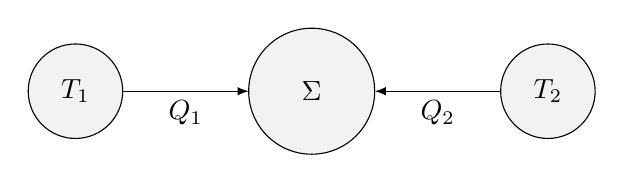
\begin{tikzpicture}
  %tikz thermo
    \draw[fill=gray!10] (0,0) circle (0.8cm) node[] {$\Sigma$ };

    \draw[fill=gray!10] (-3,0) circle (0.6cm) node[] {$T_1$ };
    \draw[fill=gray!10] (3,0) circle (0.6cm) node[] {$T_2$ };
    \draw[-latex] (-2.4, 0) -- node[below]{$Q_1$ } (-0.8, 0);
    \draw[-latex] (2.4, 0) -- node[below]{$Q_2$ } (0.8, 0);
  \end{tikzpicture}
\end{center}

\subsection{Transformation réversible}%
\label{sub:transformation_reversible}
Une transformation est qualifiée de \emph{réversible} lorsqu'elle est physiquement possible dans les deux sens. En pratiquen, pour sa voir si une transformation est réversible, il faut imaginer qu'elle est filmée puis visionnée en partant de la fin du film. Si la transformation semble physiquement possible, alors elle est réversible.

Parmi les causes d'irréversibilité d'une transformation, on peut citer
\begin{itemize}
  \item Les frottements solides ou fluides ;
  \item les différences de température ;
  \item la diffusion en général.
\end{itemize}

On notera qu'une transformation adiabatique réversible conserve l'entropie du système, on dit qu'elle est \textbf{isentropique}. Par contre ça n'est pas une condition nécessaire, une transformation peut être isentropique sans être ni adiabatique, ni réversible.

Une transformation réversible est forcément quasistatique. En effet, si un état intermédiaire de la transformation n'est pas un état d'équilibre, la transformation obtenue par renversement du temps ne n'est pas physiquement possible en ce point.

\subsection{Interprétation statistique de l'entropie}%
\label{sub:interpretation_statistique_de_l_entropie}
L'introduction de la fonction d'état entropie dans le second principe peut paraitre très artificielle, et le second principe ne fournit pas une interprétation qualitative évidente de ce que représente l'entropie.

La \textit{physique statistique} permet de donner une interprétation qualitative beaucoup plus claire de ce qu'est l'entropie. Pour comprendre comment, nous allons considérer un système très simple constitué de $N$ particules qui ne peuvent être que dans 2 états différents. Un état d'énergie nulle et un état d'énergie $E$. C'est un \textit{système à deux niveaux}. 

Macroscopiquement, il n'est pas possible de déterminer l'état individuel de chaque particule et l'état du système est totalement déterminé par son énergie interne $U$. Un état d'énergie interne $U$ donnée est appelé un \textit{macro-état}. 

Microscopiquement, on peut décrire l'état du système par la liste $E_i$ des énergies de chaque particule. Une liste des énergies des particules du système est un \textit{micro-état}.

On peut se convaincre assez facilement qu'il peut exister plusieurs micro-états conduisant au même macro-état. Sur la figure ci-dessous, on montre deux macro-états et les micro-états correspondant pour un système comportant $N=4$ particules.

\begin{center}
  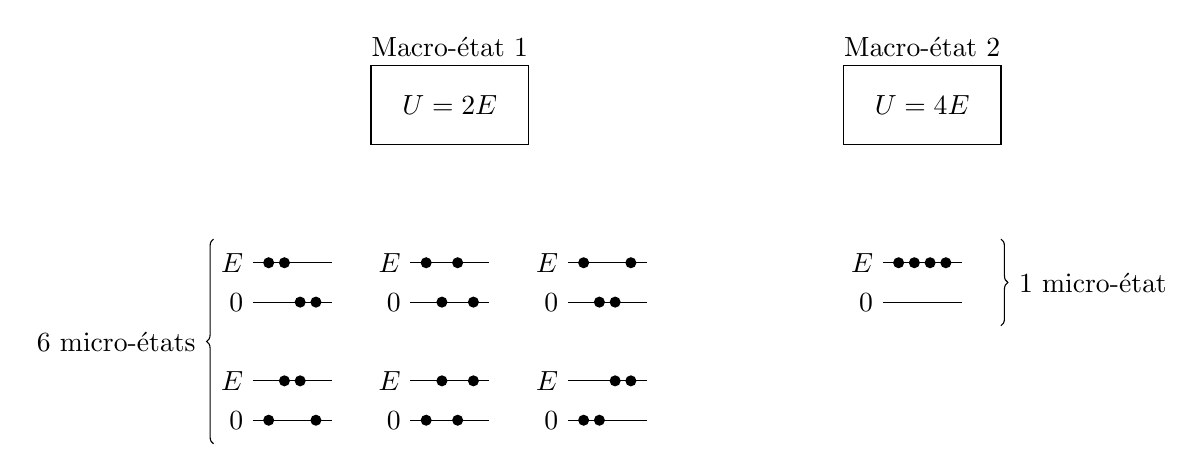
\begin{tikzpicture}
    \draw (-0.5,0) rectangle ++(2,1) (0.5,0.5) node{$U=2E$}; 
    \draw (0.5, 1) node[above]{Macro-état 1};
    \draw (5.5,0) rectangle ++(2,1) (6.5,0.5) node{$U=4E$}; 
    \draw (6.5, 1) node[above]{Macro-état 2};

    \begin{scope}[shift={(-2,-2)}]
      \draw[] (0,0) node[left]{$0$}  -- (1,0);
      \draw[] (0,0.5) node[left]{$E$} -- (1, 0.5);
      \fill (0.2, 0.5) circle (2pt); 
      \fill (0.4, 0.5) circle (2pt); 
      \fill (0.6, 0) circle (2pt); 
      \fill (0.8, 0) circle (2pt); 
    \end{scope}
    \begin{scope}[shift={(0,-2)}]
      \draw[] (0,0) node[left]{$0$}  -- (1,0);
      \draw[] (0,0.5) node[left]{$E$} -- (1, 0.5);
      \fill (0.2, 0.5) circle (2pt); 
      \fill (0.4, 0) circle (2pt); 
      \fill (0.6, 0.5) circle (2pt); 
      \fill (0.8, 0) circle (2pt); 
    \end{scope}
    \begin{scope}[shift={(2,-2)}]
      \draw[] (0,0) node[left]{$0$}  -- (1,0);
      \draw[] (0,0.5) node[left]{$E$} -- (1, 0.5);
      \fill (0.2, 0.5) circle (2pt); 
      \fill (0.4, 0) circle (2pt); 
      \fill (0.6, 0) circle (2pt); 
      \fill (0.8, 0.5) circle (2pt); 
    \end{scope}
    \begin{scope}[shift={(-2,-3.5)}]
      \draw[] (0,0) node[left]{$0$}  -- (1,0);
      \draw[] (0,0.5) node[left]{$E$} -- (1, 0.5);
      \fill (0.2, 0) circle (2pt); 
      \fill (0.4, 0.5) circle (2pt); 
      \fill (0.6, 0.5) circle (2pt); 
      \fill (0.8, 0) circle (2pt); 
    \end{scope}
    \begin{scope}[shift={(0,-3.5)}]
      \draw[] (0,0) node[left]{$0$}  -- (1,0);
      \draw[] (0,0.5) node[left]{$E$} -- (1, 0.5);
      \fill (0.2, 0) circle (2pt); 
      \fill (0.4, 0.5) circle (2pt); 
      \fill (0.6, 0) circle (2pt); 
      \fill (0.8, 0.5) circle (2pt); 
    \end{scope}
    \begin{scope}[shift={(2,-3.5)}]
      \draw[] (0,0) node[left]{$0$}  -- (1,0);
      \draw[] (0,0.5) node[left]{$E$} -- (1, 0.5);
      \fill (0.2, 0) circle (2pt); 
      \fill (0.4, 0) circle (2pt); 
      \fill (0.6, 0.5) circle (2pt); 
      \fill (0.8, 0.5) circle (2pt); 
    \end{scope}

    \draw[decorate, decoration={brace, mirror}] (-2.5, -1.2) -- (-2.5, -3.8) node[midway, left=3pt]{6 micro-états}; 

    \begin{scope}[shift={(6,-2)}]
      \draw[] (0,0) node[left]{$0$}  -- (1,0);
      \draw[] (0,0.5) node[left]{$E$} -- (1, 0.5);
      \fill (0.2, 0.5) circle (2pt); 
      \fill (0.4, 0.5) circle (2pt); 
      \fill (0.6, 0.5) circle (2pt); 
      \fill (0.8, 0.5) circle (2pt); 
    \end{scope}

    \draw[decorate, decoration={brace}] (7.5, -1.2) -- (7.5, -2.3) node[midway, right=3pt]{1 micro-état}; 

  \end{tikzpicture}
  \captionof{figure}{Représentation de deux macro-états avec les micro-états correspondants pour un système à deux niveaux comportants 4 particules.}
\end{center}

Sur cette figure, on remarque que tous les macro-états ne sont pas équivalents. Le macro-état 1 peut être atteint de 6 manières différentes alors qu'il n'y a qu'une possibilité d'atteindre le macro-état 2. 

Dit autrement, lorsque l'on dit que le système est dans le macro-état 2, on a toute l'information possible sur le système, on connait l'état de toutes les particules, on dit que c'est un état \textit{ordonné}. D'un autre côté, lorsqu'on sait que l'on se trouve dans le macro-état 2, il nous manque encore beaucoup d'information pour connaître l'état microscopique du système. On dit que c'est un état \textit{désordonné}.

Pour quantifier l'ordre d'un macro-état, on introduit \textit{l'entropie statistique} $S$ d'un macro-état définie par :  
\begin{eqencadre}
  S = k_B\ln(\Omega)
\end{eqencadre}

où $\Omega$ est le nombre de micro-états possibles. 

On peut montrer que cette définition statistique de l'entropie rejoint la définition thermodynamique que l'on a donnée dans le second principe. L'entropie est une \textit{mesure du désordre} associé à une état macroscopique.

\section{Entropie de changement d'état}%
\label{sec:entropie_de_changement_d_etat}
Considérons un système thermodynamique constitué d'un corps pur dans un état donné, par exemple liquide à sa température de changement d'état notée $T$, par exemple sa température d'ébullition.

On effectue un changement d'état du système en le mettant en contact avec un thermostat à la température $T$, par exemple, on fait passer la totalité du corps pur à l'état gazeux.

On peut effectuer ce changement d'état de façon réversible (tant que la source de chaleur est à la température $T$), dans ce cas, l'entropie créée lors de la transformation est nulle et on peut écrire la variation $\Delta S$ d'entropie du système comme
\begin{equation}
  \Delta S = S_\text{échangée} =\frac{Q}{T}
\end{equation}
Comme la température est constante, le changement d'état se fait aussi à pression constante (voire les isothermes du diagramme de Clapeyron), comme on considéré une transformation réversible, elle est aussi quasistatique et la pression du système est égale à la pression extérieure. Donc la transformation est aussi monobare. Dans ces conditions, on peut écrire
\begin{equation}
  Q = \Delta H
\end{equation}
On arrive à la relation importante entre la variation d'entropie $\Delta S$ lors du changement d'état et la variation $\Delta H$ d'enthalpie :
\begin{eqencadre}
  \Delta S = \frac{\Delta H}{T} \quad \text{ou}\quad \Delta H = T \Delta S
\end{eqencadre}
au cours d'un changement d'état.

On peut en déduire, par exemple, la relation entre l'entropie massique de fusion d'un corps pur $s_\text{fus}$ et son enthalpie massique de fusion $h_\text{fus}$ 
\begin{equation}
  h_\text{fus} = T s_\text{fus}
\end{equation}
où $T$ est la température de fusion.


\section{Variation d'entropie d'un gaz parfait (hors programme)}%
\label{sec:variation_d_entropie_d_un_gaz_parfait}

Nous allons déterminer la variation d'entropie de $n$ moles d'un gaz parfait au cours d'une transformation qui le fait passer d'un état $(p_1, V_1, T_1)$ à un état $(p_2, V_2, T_2)$. Ces trois paramètres ne sont pas indépendants et on a 
\begin{equation}
  p_1V_1 = nRT_1 \quad \text{et}\quad p_2V_2 =nRT_2.
\end{equation}
On ne s'intéressera plus qu'aux variables $p$ et $T$. 

Comme l'entropie est un fonction d'état, on peut choisir n'importe quel chemin entre ces deux états. Pour pouvoir calculer facilement la variation d'entropie, on choisira un chemin réversible que l'on décomposera en deux étapes :
\begin{itemize}
  \item Première étape : on change la température du gaz à pression constante pour passer de $(p_1, T_1)$ à $(p_1, T_2)$ ;
  \item deuxième étape : on change la pression à température constante pour passer de $(p_1, T_2)$ à $(p_2, T_2)$.  
\end{itemize}
Ces deux transformations seront faites de manière réversible, de telle sorte que $S_\text{c}=0$ et donc $\Delta S = S_\text{e}$. 

Au cours de la première étape, on aimerait bien écrire 
\begin{equation}
  \Delta S_1 = S_\text{e} = \frac{Q_1}{T}
\end{equation}
mais ça n'est pas possible car la température varie au cours de la transformation. On va donc décomposer la transformation en une infinité de \emph{transformations élémentaires} au cours desquelles la température pourra être considérée constante. Au cours d'une transformation élémentaire, le système reçoit un transfert thermique $\delta Q$ et son entropie varie de $\D S$. On a alors 
\begin{equation}
  \D S = \frac{\delta Q}{T} = \frac{C_p\D T}{T}\,.
\end{equation}
%
Car la transformation se fait à pression constante, et on peut écrire la chaleur $\delta Q$ reçue comme $\delta Q = C_p \D T$. On trouve alors la variation d'entropie $\Delta S_1$ au cours de cette première étape en faisant la somme de toutes les variations d'entropie élémentaires
\begin{equation}
  \Delta S_1 = \int_{T_1}^{T_2}\D S = \int_{T_1}^{T_2}\frac{C_p}{T}\D T = C_p \ln \left( \frac{T_2}{T_1} \right) 
\end{equation}

La deuxième étape se fait à température constante, donc on peut écrire 
\begin{equation}
 \Delta S_2 = \frac{Q_2}{T_2} 
\end{equation}
Comme c'est une transformation à température constante d'un gaz parfait, on a aussi 
\begin{equation}
  \Delta U_2 = 0 = W_2 + Q_2 \Leftrightarrow Q_2 = -W_2
\end{equation}
On cherche donc le travail $W_2$ reçu lors d'une transformation isotherme du gaz parfait. Nous l'avons déjà fait (voir chapitre~\ref{chap:premier_principe}, partie \ref{sub:application_premier_principe}) et nous avions trouvé :
\begin{equation}
  Q_2 = -nRT_2\ln \left( \frac{p_2}{p_1} \right) .
\end{equation}
Donc on a finalement
\begin{equation}
  \Delta S_2 = \frac{Q_2}{T_2} = -nR\ln \left( \frac{p_2}{p_1} \right) 
\end{equation}
On introduit $\gamma = \frac{C_p}{C_V}$ et avec la relation de Mayer, on peut montrer que $C_p = \frac{\gamma nR}{\gamma-1}$ et donc la variation d'entropie au cours de la transformation globale devient
\begin{equation}
  \Delta S = \Delta S_1 + \Delta S_2 = \frac{nR}{\gamma -1}\left[ \gamma\ln\left(  \frac{T_2}{T_1}\right) - (\gamma -1)\ln\left( \frac{p_2}{p_1} \right)  \right] 
\end{equation}
Avec l'équation d'état des gaz parfaits, on obtient finalement
\begin{equation}
  \Delta S = \frac{nR}{\gamma -1}\ln \left( \frac{p_2V_2^\gamma}{p_1V_1^\gamma} \right) 
\end{equation}

\end{document}
